%!TEX program = xelatex
\documentclass[UTF8,zihao=-4,fontset=adobe]{ctexbook}
% \documentclass[UTF8,zihao=-4]{ctexbook}
\usepackage[superscript]{cite}
\newcommand{\upcite}[1]{\textsuperscript{\textsuperscript{
\citeleft}\cite{#1}\textsuperscript{\citeright}}}					% 设置参考文献序号格式
%\renewcommand{\cite}[1]{\textsuperscript{\textsuperscript{
%\citeleft}\cite{#1}\textsuperscript{\citeright}}}					% 设置参考文献序号格式
% \usepackage{natbib}
% \citestyle{nature} % Superscript citation style (Nature style)

\usepackage{amsmath}
\usepackage{graphicx}
\usepackage{tikz}
\usepackage{amsthm}

\usetikzlibrary{shapes,backgrounds}
\usetikzlibrary{arrows, decorations.pathmorphing, backgrounds, positioning, fit, petri, automata} %自动机

\usetikzlibrary{matrix,arrows}


\usepackage{multirow} % 合并表格


% \usepackage{tocloft}
\usepackage{titletoc}

%%% 一些环境重定义

% \newcommand*{\artxifcnt}[1]{% check if counter exists
%     \ifcsname c@#1\endcsname%
%         \expandafter\@firstoftwo%
%     \else%
%         \expandafter\@secondoftwo%
%     \fi
% }

% \artxifcnt{chapter}{\def\artxmaincnt{chapter}}{\def\artxmaincnt{section}}%

\newtheorem{definition}{定义}[chapter]

\newtheorem{example}{例}[chapter]

\newtheorem{proposition}{惯例}[chapter]

\newtheorem{remark}{注}[chapter]

\usepackage{bicaption}
% \bicaptionsetup{font={\small}}
\usepackage{caption}
\captionsetup{font={small}}   %% 设置图标标题为 宋体五号字

\usepackage{stmaryrd}  % \talloblong

\graphicspath{{image/}}



%中英文字体设置
% \setCJKmainfont{SimSun}
% \setCJKmonofont{SimSun}
% \setmainfont{Times New Roman}
%%\normalsize{}

% \setCJKmainfont{SimSun}
% \setCJKmonofont{SimSun}
% \setmainfont{Times New Roman}
% \setCJKfamilyfont{zhsong}{SimSun}
% \renewcommand*{\songti}{\CJKfamily{zhsong}}

\setCJKmainfont{AdobeSongStd-Light}[AutoFakeBold,ItalicFont=AdobeKaitiStd-Regular]%
\setCJKsansfont{AdobeHeitiStd-Regular}[AutoFakeBold]%
\setCJKmonofont{AdobeFangsongStd-Regular}%
\setmainfont[NFSSFamily=entextrm]{Times New Roman}% 
\setsansfont[NFSSFamily=entextsf]{Times New Roman}% 

\newcommand{\chuhao}{\fontsize{42pt}{\baselineskip}\selectfont}     %初号
\newcommand{\xiaochuhao}{\fontsize{36pt}{\baselineskip}\selectfont} %小初号
\newcommand{\yihao}{\fontsize{28pt}{\baselineskip}\selectfont}      %一号
\newcommand{\erhao}{\fontsize{21pt}{\baselineskip}\selectfont}      %二号
\newcommand{\xiaoerhao}{\fontsize{18pt}{\baselineskip}\selectfont}  %小二号
\newcommand{\sanhao}{\fontsize{15.75pt}{\baselineskip}\selectfont}  %三号
\newcommand{\sihao}{\fontsize{14pt}{\baselineskip}\selectfont}%     四号
\newcommand{\xiaosihao}{\fontsize{12pt}{\baselineskip}\selectfont}  %小四号
\newcommand{\wuhao}{\fontsize{10.5pt}{\baselineskip}\selectfont}    %五号
\newcommand{\xiaowuhao}{\fontsize{9pt}{\baselineskip}\selectfont}   %小五号
\newcommand{\liuhao}{\fontsize{7.875pt}{\baselineskip}\selectfont}  %六号
\newcommand{\qihao}{\fontsize{5.25pt}{\baselineskip}\selectfont}    %七号


\ctexset {
    chapter = {
        % format = \linespread{1.0}\zihao{3}\bfseries\heiti\centering,
        format = \linespread{1.0}\zihao{3}\heiti\centering,
        nameformat = {},
        titleformat = {},
        number = \chinese{chapter},
        numberformat = \heiti,
        aftername = \quad,
        beforeskip = {7pt},
        afterskip = {18pt},
        pagestyle = plain,
    }
}
%- section
\ctexset {
    section = {
        % format = \linespread{1.0}\zihao{4}\bfseries\centering,
        format = \linespread{1.0}\zihao{4}\centering,
        numberformat = \rmfamily,
        aftername = \quad,
        beforeskip = {24pt},
        afterskip = {6pt},
    }
}
%- subsection
\ctexset {
    subsection = {
        % format = \linespread{1.0}\zihao{-4}\bfseries\raggedright,
        format = \linespread{1.0}\zihao{-4}\raggedright,
        numberformat = \rmfamily,
        aftername = \quad,
        beforeskip = {12pt},
        afterskip = {6pt},
    }
}
%- subsubsection
% \ctexset {
%     subsubsection = {
%         format = \linespread{1.0}\zihao{-4}\CJKfamily{song}\raggedright,
%         numberformat = \rmfamily,
%         aftername = \quad,
%         beforeskip = {12pt},
%         afterskip = {6pt},
%     }
% }

%- appendix
\ctexset {
    appendix = {
        numbering = true, %true|false,
        number = \rmfamily\Alph{chapter},
    }
}

%% 页面设置
\usepackage{geometry}
\geometry{papersize={21.0cm,29.7cm}}
\geometry{left=3.18cm,right=3.18cm,top=2.54cm,bottom=2.54cm}

\title{有限自动机C++工具箱\\等价性和最小化类软件测试}
\author{胡双朴}
\date{2019.06}

\tolerance=1
\emergencystretch=\maxdimen
\hyphenpenalty=10000
\hbadness=10000

%% 下划线
\usepackage{ulem}









%%%%%%%%%%%% 页眉页脚格式
\usepackage{fancyhdr}
% \pagestyle{headings}
\pagestyle{fancy}
\fancyhead{}%清除页眉格式
\fancyfoot{}%清除页脚格式
\fancyhead[RO,LE]{\songti\zihao{-5}\thepage}%在奇数页右侧、偶数页左侧(也就是页面的外侧)设置页码 宋体小五。
\fancyhead[CO]{\songti\zihao{5}{\leftmark}}%奇数页页眉中心设置章次和章标题 宋体五号
\fancyhead[CE]{\songti\zihao{5}有限自动机C++工具箱等价性和最小化类软件测试}%偶数页页眉中心设置论文的题目
\renewcommand{\headrulewidth}{0.75pt} % 页眉与正文之间的水平线粗细
\renewcommand{\headwidth}{\textwidth} % 页眉与正文之间水平线的宽度
% \renewcommand{\footrulewidth}{0pt} %    
% \renewcommand{\chaptermark}[1]{\markboth{~第~\chinese{chapter}~章~~~#1~}{}}
\renewcommand{\chaptermark}[1]{\markboth{\chaptername\ \ #1}{}}
% \renewcommand{\chaptermark}[1]{\markboth{\if@mainmatter\chaptername\ \thechapter~~\fi#1}{}}
\fancypagestyle{plain}{  % 章节标题页页眉
    \pagestyle{fancy}
}
%\thispagestyle{plain}   
%\fancyhf{}






% %%%%%%%  公式编号   from https://tex.stackexchange.com/questions/61756/how-to-change-equation-numbering-style
\makeatletter
\long\def\theequation{\ifnum \c@chapter > \z@ \thechapter --\fi \@arabic \c@equation}
\makeatother
% \usepackage{etoolbox}
% \patchcmd{\theequation}{.}{--}{}{}

%%%%% 超链接
\usepackage[colorlinks,linkcolor=black,anchorcolor=blue,citecolor=red]{hyperref}


%%%%%%% 代码样式
\usepackage{listings}
\usepackage{lipsum}
%\usepackage{courier}
\usepackage{xhfill}
\usepackage{color}
\definecolor{codegreen}{rgb}{0,0.6,0}
\definecolor{codegray}{rgb}{0.5,0.5,0.5}
\definecolor{codepurple}{rgb}{0.58,0,0.82}
\definecolor{backcolour}{rgb}{0.99,0.99,1.0}

\lstdefinestyle{mystyle}{
    backgroundcolor=\color{white},   
    commentstyle=\color{codegreen},
    keywordstyle=\color{magenta},
    numberstyle=\tiny\color{codegray},
    stringstyle=\color{codepurple},
    %basicstyle=\footnotesize\sffamily,
    basicstyle=\footnotesize\ttfamily,
    breakatwhitespace=false,         
    breaklines=true,                 
    captionpos=b,                    
    keepspaces=true,                 
    numbers=left,                    
    numbersep=5pt,                  
    showspaces=false,                
    showstringspaces=false,
    showtabs=false,                  
    tabsize=2
}

\lstset{style=mystyle}
\renewcommand\lstlistingname{代码}

\begin{document}

实例化如图 \ref{fig:a-sample} 所示的DFA,测试代码如代码 \ref{lst:a-sample} 所示

% \begin{figure}
	% \centering
	% 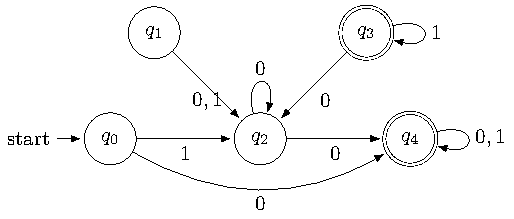
\includegraphics[width=0.8\textwidth]{automaton.tex}
	% \caption{}
	% \label{fig:a-sample}
% \end{figure}

\begin{figure}[!htbp]
	\centering
	\resizebox {0.9\textwidth} {!} {
		\begin{tikzpicture}[>=latex, shorten >=2pt,node distance=1in, on grid, auto]
			\node[state,initial] (q0) {$q_0$};
			\node[state] (q2) [right=of q0] {$q_2$};
			\node[state,accepting] (q4) [right=of q2] {$q_4$};
			\node[state] (q1) [above left=of q2] {$q_1$};
			\node[state,accepting] (q3) [above right=of q2] {$q_3$};
			\path[->]
			(q0) edge [below,bend right] node {$0$} (q4)
			(q2) edge [below] node {$0$} (q4)
			(q0) edge [below] node {$1$} (q2)
			(q1) edge [below] node {$0,1$} (q2)
			(q3) edge node {$0$} (q2)
			(q2) edge [loop above] node {$1$} (q2)
			(q4) edge [loop right] node {$0,1$} (q4)
			(q3) edge [loop right] node {$1$} (q3)
			;
		\end{tikzpicture}
    }
	\caption{}
	\label{fig:a-sample}
\end{figure}

\begin{lstlisting}[language=C++,label={lst:a-sample},caption={图 \ref{fig:a-sample} 中的DFA}]
void minDFATest3()
{
	DFA_components dfa_com1;

	// StateSet S  开始状态集
	dfa_com1.S.set_domain(5);
	dfa_com1.S.add(0);

	// StateSet F  结束状态集
	dfa_com1.F.set_domain(5);
	dfa_com1.F.add(3);
	dfa_com1.F.add(4);

	int i = 5;
	while (i--)
	{
		dfa_com1.Q.allocate();
	}

	dfa_com1.T.set_domain(5);
	dfa_com1.T.add_transition(0, '0', 4);
	dfa_com1.T.add_transition(0, '1', 2);
	dfa_com1.T.add_transition(1, '0', 2);
	dfa_com1.T.add_transition(1, '1', 2);
	dfa_com1.T.add_transition(2, '0', 4);
	dfa_com1.T.add_transition(2, '1', 2);
	dfa_com1.T.add_transition(3, '0', 2);
	dfa_com1.T.add_transition(3, '1', 3);
	dfa_com1.T.add_transition(4, '0', 4);
	dfa_com1.T.add_transition(4, '1', 4);

	//实例化一个DFA对象
	DFA dfa1(dfa_com1);
	cout << "\n************ DFA\n" << std::flush;
	cout << dfa1 << endl;

	dfa1.usefulf();  // 没有删除1,3 ?
	cout << dfa1 << endl;
	cout << " is the DFA Usefulf ?: " << dfa1.Usefulf() << endl;

	dfa1.min_Hopcroft();
	cout << "\n************ minDFA\n" << std::flush;
	cout << dfa1 << endl;
}
\end{lstlisting}

代码 \ref{lst:a-sample} 将输出如下信息

\begin{lstlisting}[language=C++,label={lst:a-sample-result},caption={图 \ref{fig:a-sample} 中的DFA 在算法 Hopcroft 算法中的输出}]
************ DFA

DFA
Q = [0,5)
S = { 0 }
F = { 3  4 }
Transitions =
0->{ '0'->4  '1'->2 }
1->{ ['0','1']->2 }
2->{ '0'->4  '1'->2 }
3->{ '0'->2  '1'->3 }
4->{ ['0','1']->4 }

current = -1


DFA
Q = [0,5)
S = { 0 }
F = { 3  4 }
Transitions =
0->{ '0'->4  '1'->2 }
1->{ ['0','1']->2 }
2->{ '0'->4  '1'->2 }
3->{ '0'->2  '1'->3 }
4->{ ['0','1']->4 }

current = -1

 is the DFA Usefulf ?: 1

************ minDFA

DFA
Q = [0,4)
S = { 0 }
F = { 2  3 }
Transitions =
0->{ '0'->3  '1'->0 }
1->{ ['0','1']->0 }
2->{ '0'->0  '1'->2 }
3->{ ['0','1']->3 }
current = -1
\end{lstlisting}

本例中,$q_1$和$q_3$都不是 \verb+final-unreachable+ (陷阱)状态,所以不会在执行函数 \verb+DFA::usefulf()+ 后去除。

执行最小化算法 \verb+DFA::min_Hopcroft+ 后的 DFA 如图 \ref{fig:a-sample-error} 所示。

\begin{figure}[!htbp]
	\centering
	\resizebox {0.6\textwidth} {!} {
		\begin{tikzpicture}[>=latex, shorten >=2pt,node distance=1in, on grid, auto]
			\node[state,initial] (q0) {$q_0$};
			\node[state,accepting]  [right=of q0] (q3) {$q_3$};
			\node[state,accepting]  [above=of q3] (q2) {$q_2$};
			\node[state] [left =of q2] (q1) {$q_1$};
			\path[->]
			(q0) edge [below] node {$0$} (q3)
			(q0) edge [loop below] node {$1$} (q0)
			(q1) edge  node {$0,1$} (q0)
			(q2) edge [below] node {$0$} (q0)
			(q2) edge [loop right] node {$1$} (q2)
			(q3) edge [loop right] node {$0,1$} (q3)
			;
		\end{tikzpicture}
    }
	\caption{}
	\label{fig:a-sample-error}
\end{figure}

经过测试,算法\verb+DFA::min_dragon+,\verb+DFA::min_Watson+,\verb+DFA::min_HopcroftUllman+的输出与算法\verb+DFA::min_Hopcroft+相同。而算法\verb+DFA::min_Brzozowski+的输出为
\begin{lstlisting}[language=C++,label={lst:a-sample-Brzozowski},caption={图 \ref{fig:a-sample} 中的DFA 在算法 Hopcroft 算法中的输出}]
************ DFA
DFA
Q = [0,2)
S = { 0 }
F = { 1 }
Transitions =
0->{ '0'->1  '1'->0 }
1->{ ['0','1']->1 }

current = -1
\end{lstlisting}

对应的状态转移图为图 \ref{fig:a-sample-bbb}

\begin{figure}[!htbp]
	\centering
	\resizebox {0.5\textwidth} {!} {
		\begin{tikzpicture}[>=latex, shorten >=2pt,node distance=1in, on grid, auto]
			\node[state,initial] (q0) {$q_0$};
			\node[state,accepting]  [right=of q0] (q1) {$q_1$};
			\path[->]
			(q0) edge [below] node {$0$} (q1)
			(q0) edge [loop above] node {$1$} (q0)
			(q1) edge [loop above] node {$0,1$} (q1)
			;
		\end{tikzpicture}
    }
	\caption{}
	\label{fig:a-sample-bbb}
\end{figure}

\newpage

{\bfseries 结论}

对于图 \ref{fig:a-sample} 中的自动机,仅有算法 \verb+DFA::min_Brzozowski+输出了正确的结果,\verb+DFA::min_Hopcroft+无论是否经过修改,均输出错误结果。

对于图 \ref{fig:a-sample} 中的自动机,移除状态$q_3$之后,之前错误的算法也能输出正确结果。

\begin{remark}
除了算法\verb+DFA::min_Brzozowski+外,其他算法均不能移除自动机中的开始不可达状态。
\end{remark}

增加对其他算法的测试后的代码如下
\begin{lstlisting}[language=C++,label={lst:a-sample-addtion},caption={}]
void minDFATest3()
{
	DFA_components dfa_com1;

	// StateSet S  开始状态集
	dfa_com1.S.set_domain(5);
	dfa_com1.S.add(0);

	// StateSet F  结束状态集
	dfa_com1.F.set_domain(5);
	dfa_com1.F.add(3);
	dfa_com1.F.add(4);

	int i = 5;
	while (i--)
	{
		dfa_com1.Q.allocate();
	}

	dfa_com1.T.set_domain(5);
	dfa_com1.T.add_transition(0, '0', 4);
	dfa_com1.T.add_transition(0, '1', 2);
	dfa_com1.T.add_transition(1, '0', 2);
	dfa_com1.T.add_transition(1, '1', 2);
	dfa_com1.T.add_transition(2, '0', 4);
	dfa_com1.T.add_transition(2, '1', 2);
	dfa_com1.T.add_transition(3, '0', 2);
	dfa_com1.T.add_transition(3, '1', 3);
	dfa_com1.T.add_transition(4, '0', 4);
	dfa_com1.T.add_transition(4, '1', 4);

	//实例化一个DFA对象
	DFA dfa1(dfa_com1);
	cout << "\n************ DFA\n" << std::flush;
	cout << dfa1 << endl;

	cout << " is the DFA Usefulf ?: " << dfa1.Usefulf() << endl;
	dfa1.usefulf();  // 没有删除1,3 ?
	cout << dfa1 << endl;
	cout << " is the DFA Usefulf ?: " << dfa1.Usefulf() << endl;

	dfa1.min_Hopcroft();
	cout << "\n************ minDFA (Hopcroft) \n" << std::flush;
	cout << dfa1 << endl;


	//增加对其他最小化算法的测试
	DFA dfa2(dfa_com1);
	dfa2.min_Brzozowski();
	cout << "\n************ minDFA (Brzozowski)\n" << std::flush;
	cout << dfa2 << endl;

	DFA dfa3(dfa_com1);
	dfa3.usefulf();
	dfa3.min_dragon();
	cout << "\n************ minDFA (dragon) \n" << std::flush;
	cout << dfa3 << endl;

	DFA dfa4(dfa_com1);
	dfa4.usefulf();
	dfa4.min_HopcroftUllman();
	cout << "\n************ minDFA (HopcroftUllman) \n" << std::flush;
	cout << dfa4 << endl;

	DFA dfa5(dfa_com1);
	dfa5.usefulf();
	dfa5.min_Watson();
	cout << "\n************ minDFA (Watson)\n" << std::flush;
	cout << dfa5 << endl;
}
\end{lstlisting}

% \thispagestyle{empty}
% \maketitle
% \thispagestyle{empty}

% %%%%%%%%%%%%% 目录开始  %%%%%%%%%%%%%
% \cleardoublepage
% \pagenumbering{Roman}  %-- 设置罗马数字
% \setcounter{page}{1}
% \pdfbookmark[1]{\contentsname}{toc}
% \tableofcontents
% \titlecontents{chapter}[4em]{\bfseries \zihao{-4} \vspace{10pt}}{\contentslabel{4em}}{\hspace*{-4em}}{~\titlerule*[1pc]{$.$}~\contentspage}
% % \tableofcontents{section}[4em]{\bfseries \zihao{5} \vspace{10pt}}{\contentslabel{4em}}{\hspace*{-4em}}{~\titlerule*[0.6pc]{$.$}~\contentspage}

% %%%%%%%%%%%%%%   为目录添加一页空白页  %%%%%%%%%%%%%%%%

% %\newpage
% % \thispagestyle{empty}
% % \clearpage
% % \phantom{s}
% % % \newpage
% % \thispagestyle{empty}

% %%%%%%%%%%%%% 目录结束  %%%%%%%%%%%%%

% %\newpage

 % %-- 重新开始目录编号

% \cleardoublepage
% \renewcommand\chaptername{~第~\chinese{chapter}~章~}
% \input{yinyan.tex}
% \pagenumbering{arabic}
% \setcounter{page}{1}
% \input{preliminaries.tex}
% \input{equivalent_relation.tex}
% \input{construct_DFA.tex}
% \input{realwork.tex}

% % -- 参考文献
% % % \bibliographystyle{gbt7714-2005}
% % \bibliographystyle{ieeetr}
% \bibliographystyle{XDUbib}
% {\zihao{5}  %%% 修改参考文献页面字体大小为 5 号字体

% \bibliography{ref}

% }

% \addcontentsline{toc}{chapter}{参考文献}

% % -- 附录
% %\appendix
% \begin{appendix}
% \renewcommand\chaptername{附录~\thechapter{}~}
% %!TEX root = ../Demo.tex
% \chapter*{A 一些基本定义}
% \addcontentsline{toc}{chapter}{A 一些基本定义}
\chapter{一些基本定义}

\begin{convention}[幂集] 
    对于任意集合$A$,我们使用$\mathcal{P}(A)$代表$A$的所有子集。$\mathcal{P}(A)$也叫做$A$的幂集。有时也写作 $2^A$。
\end{convention}

\begin{convention}[函数集] \label{pro:mathP}
    对于集合 $A$ 和 $B$ ,$A\to B$代表所有从$A$到$B$的函数的集合。而 $ A \not\to B$代表所有从$A$到$B$的“partial functions”。
\end{convention}


\begin{remark}
    对于集合$A,B$,关系 $\mathcal{C}\subseteq A \times B$ ,我们可以把$\mathcal{C}$理解为函数 $\mathcal{C} \in A \longrightarrow \mathcal{P}(B)$。
\end{remark}



\begin{convention}[元组投影]
    对于$n$元组 $t=(x_1,x_2,\cdots,x_n)$,我们使用符号${\pi}_i(t)$ $(1 \leq i \leq n)$ 代表元组元素$x_i$;我们使用符号 $\bar{\pi}_i(1 \leq i \leq n)$代表$(n\mbox{-}1)$元组$(x_1,\cdots,x_{i-1},x_{i+1},\cdots,x_n)$。$\pi$ 和 $\bar{\pi}$ 自然扩展到元组集。 
\end{convention}



\begin{convention}[组合关系]
    给出集合$A,B,C$和两个关系$E \subseteq A \times B$ 和 $ F \subseteq B \times C $,定义组合关系(插入操作符$\circ$):
$$ E\circ F = \{ (a,c) : (\exists b:b \in B : (a,b) \in E \land (b,c) \in F) \} $$ 
\end{convention}



\begin{convention}[等价关系的等价类]
    对任何集合 $A$ 上的等价关系 $E$,我们使用 $[A]_E$代表等价类集合,即:
$$ [A]_E = \{ [a]_E :a \in A \} $$
集合 $[A]_E$ 也叫做 $A$ 的由 $E$ 引出的“划分(partition)”。
\end{convention}


\begin{definition}[等价类的指数]
    对于集合$A$上的等价关系$E$,定义$\sharp E = | [A]_E |$。$\sharp E$ 也叫做$E$的“指数”。
\end{definition}


\begin{definition}[字母表] \label{def:Alphabat}
    字母表是有限大小的非空集合。
\end{definition}



\begin{definition}[等价关系的细化]
    对于等价关系$E$和$E'$(在集合$A$上),当且仅当$E \subseteq E'$,$E$是$E'$的“细化”。
\end{definition}

\begin{definition}[划分的细化关系$\sqsubseteq$]
    对于等价关系$E$和$E'$(在集合$A$上),当且仅当$ E \subseteq E' $, $[A]_E$也被称为$ [A]_{E'} $的细化(写作$ [A]_E \sqsubseteq [A]_{E'} $)。当且仅当 $E$ 下的每一个等价类完全包含在$E'$下的某些等价类时,等价命题是$ [A]_E \sqsubseteq [A]_{E'} $ 。
\end{definition}


\begin{definition}[元组和关系反转]
    对一个$n$元组$(x_1,x_2,\cdots,x_n)$,定义反转为函数$R$(后缀和上标)
    $$ (x_1,x_2,\cdots,x_n)^R = (x_n,\cdots,x_2,x_1) $$
给出一个集合元组$A$,定义$A^R = \{ x^R:x\in A \}$。
\end{definition}



% \section*{B 有限自动机($FA$)}
\addcontentsline{toc}{section}{B 有限自动机($FA$)}

本节中我们定义有限自动机、其性质及其一些变化。大部分定义直接取自 \cite{Wats93}。
\newline

\noindent{\textbf{定义 B.1(有限自动机($FA$))}: 一个自动机拥有6个元组$(Q,V,T,E,S,F)$,其中

\begin{itemize}
    \item[·] $Q$ 是有限状态集;
    \item[·] $V$ 是一个字母表;
    \item[·] $ T \in \mathcal{P}(P\times V \times Q) $是一个转换关系;
    \item[·] $ E \in \mathcal{P}(Q\times Q)$ 是一个 $\epsilon$-转换关系;
    \item[·] $ S \subseteq Q $是开始状态集;
    \item[·] $ F \subseteq Q $是结束状态集;     
\end{itemize}
字母表和函数$\mathcal{P}$的定义分别在“定义 A.8” 和 “惯例 A.1”。
\newline

\noindent{\textbf{备注 B.2}: we will take some liberty in our interpretation of the signatures of the transition relations。例如,我们也使用signature $T\in V \longrightarrow \mathcal{P}(Q\times Q),T\in Q \times Q \longrightarrow \mathcal{P}(V),T\in Q \times V \longrightarrow \mathcal{P}(Q),T\in Q \longrightarrow \mathcal{P}(V\times Q),E\in Q \longrightarrow \mathcal{P}(Q)$。每种情况下,$Q$的从左到右的顺序会是“preserved”;例如,函数$T\in Q \longrightarrow \mathcal{P}(V \times Q)$ 定义为 $T(p)=\{ (a,q) : (p,a,q) \in T \}$。所使用的签名将从上下文中清除。详见备注 A.3。$\longrightarrow$ 出现在惯例 A.2。

由于本文中我们只考虑有限自动机,所以我们将会频繁的使用简化词汇自动机。

%%%%%%%%%%%%%%%%%%%%%%%%%%%%%%%%%%%%%%%%%%%%%%%%%%%%%%%%%%%%%
\subsection*{B.1 $FA$的性质}
\addcontentsline{toc}{subsection}{B.1 有限自动机的性质}
本小节将会定义一些有限自动机的性质。为了使定义更加简洁明了,我们引进三个特殊的$FA$: $M=(Q,V,T,E,S,F)$,$M_0=(Q_0,V_0,T_0,E_0,S_0,F_0)$,$ M_1=(Q_1,V_1,T_1,E_1,S_1,F_1) $。

\noindent{\textbf{定义 B.3(FA的大小)}:定义一个FA的大小为$|M|=|Q|$}。
\newline

\noindent{\textbf{定义 B.4(FA的同构$\cong$)}:我们把同构定义为FA的等价关系}。当且仅当 $V_0=V_1$,并且存在双射$g\in Q_0 \longrightarrow Q_1$ 

\begin{itemize}
    \item[·] $T_1 = \{ (g(p,q),a,g(q)) : (p,a,q) \in T_0 \}$,
    \item[·] $E_1 = \{ (g(p,q),a,g(q)) : (p,q) \in E_0\}$,
    \item[·] $S_1 = \{ g(s):s\in S_0 \}$,and 
    \item[·] $F_1 = \{ g(f):f\in F_0 \}$
\end{itemize}
时$M_0$和$M_1$是同构的(写作$M_0 \cong M_1$)。
\newline

\noindent{\textbf{定义 B.5(转换关系$T$的扩展)}: 我们把$T \in V \longrightarrow \mathcal{P} (Q \times Q) $ 到 $ T* \in V* \longrightarrow \mathcal{P} (Q \times Q)  $的转换关系以如下方式扩展: } \\
\mbox{  } $T*(\epsilon) = E*$ \\
\mbox{and for } $(a\in V,w\in V*)$ \\
\mbox{  } $ T*(aw) = E* \circ T(a) \circ T*(w) $ \\
操作符$\circ$在惯例 4.5 中定义。This definition could also have been presented symmetrically.
\newline

\noindent{\textbf{备注 B.6}:有时候我们也使用 signatures $T* \in Q \times Q \longrightarrow \mathcal{P}(V*)$}
\newline

\noindent{\textbf{定义 B.7(左语言和右语言)}:状态(M中)的做语言由函数$ \overleftarrow{\mathcal{L}} _M \in Q \longrightarrow \mathcal{P}(V*)$,其中} \\
\mbox{  } $ \overleftarrow{\mathcal{L}}_M (q) = ( \cup s:s \in S : T*(s,q) ) $ \\
状态($M$中)的右语言由函数$ \overrightarrow{\mathcal{L}} _M \in Q \longrightarrow \mathcal{P}(V*)$给出,其中 \\
\mbox{  } $ \overrightarrow{\mathcal{L}}_M (q) = ( \cup s:s \in S : T*(s,q) ) $ \\
通常在没有歧义的时候移除下标$M$。
\newline

\noindent{\textbf{定义 B.8(FA的语言)}:有限自动机的语言由函数 $\mathcal{L}_{FA} \in FA \longrightarrow \mathcal{P}(V*) $给出,该函数的定义为:} \\
\mbox{  } $ \mathcal{L}_{FA} (M) = (\cup s,f:s \in S \land f \in F : T* (s,f)) $ \\

\noindent{\textbf{定义 B.9($Complete$)}: 一个完全小化自动机满足 : } \\
\mbox{  } $ Complete(M) \equiv ( \forall q,a:q\in Q \land a \in V : T(q,a) \not= \emptyset )$ \\

\noindent{\textbf{定义 B.10 ($\epsilon$-$free$)}: 当且仅当 $E=\emptyset$时,M 是 $\epsilon$-$free$ 的。
\newline

\noindent{\textbf{定义 B.11(初始可行自动机)}:一个 $Useful_s$ 有限自动机定义如下:} \\
\mbox{  } $ Useful_s (M) \equiv ( \forall q:q \in Q : \overleftarrow{\mathcal{L}} (q) \not= \emptyset ) $ \\

\noindent{\textbf{定义 B.12(最终可行自动机)}:一个 $Useful_f$ 有限自动机定义如下:} \\
\mbox{  } $ Useful_f (M) \equiv ( \forall q:q \in Q : \overleftarrow{\mathcal{L}} (q) \not= \emptyset ) $ \\

\noindent{\textbf{备注 B.13}: $Useful_s$和$Useful_f$与 $FA$ 的反转密切相关(见变换 B.22),对所有的 $M \in FA$,有 $Useful_f (M) \equiv Useful_s (M^R)$。 \\

\noindent{\textbf{定义 B.14(Useful 自动机)}:$Useful$自动机是一个 with only reachable states:  }\\
\mbox{  } $ Useful (M) \equiv Useful_s (M) \land Useful_f (M) $ \\

\noindent{\textbf{性质 B.15(确定性有限自动机($DFA$))}:当且仅当 }
\begin{itemize}
    \item [·] 无多重初始状态;
    \item [·] 无$\epsilon$转移;
    \item [·] 转移函数$T \in Q \times V \longrightarrow \mathcal{P} (Q) $ 不将 $Q \times V$ 中的“对”映射至多重状态。
\end{itemize}
时有限自动机$M$是确定性的。\\
形式表达为:
$$ Det(M) \equiv ( |S| \leq 1 \land \epsilon-free(E) \land ( \forall q,a:q \in Q \land a \in V : |T(q,a)| \leq 1 )) $$

\noindent{\textbf{定义 B.16($FA$的确定性)}:$DFA$代表所有确定性的有限自动机的集合。我们把$FA \setminus DFA$称为非确定性有限自动机的集合。} \\

\noindent{\textbf{惯例 B.17(DFA的转换函数)}:对于$(Q,V,T,\emptyset,S,F)\in DFA$,我们考虑把转换函数记为$T\in Q \times V \not\rightarrow Q$($\not\rightarrow$的定义可以查看惯例A.2)。当且仅当$DFA$是完全的时候,转换函数是全函数。} \\

\noindent{\textbf{性质 B.18(弱确定性自动机)}:一些作者用比$Det$弱的确定性自动机的定义;使用左语言,定义如下:}
$$ Det'(M) \equiv (\forall q_0,q_1 : q_0 \in Q \land q_1 \in Q \land q_0 \not= q_1 : \overleftarrow{\mathcal{L}}(q_0) \cap \overleftarrow{\mathcal{L}}(q_1) = \emptyset ) $$
很容易证明$Det(M) \Rightarrow Det'(M)$。
\newline

\noindent{\textbf{定义 B.19($DFA$的最小化)}:满足以下条件时,$M\in DFA$是最小化的:}
$$ Min(M) \equiv (\forall M' : M' \in DFA \land \mathcal{L}(M) = \mathcal{L}_{FA}(M') : |M| \leq |M'| ) $$
$Min$仅定义在$DFA$上。如果我们定义一个最小的但是仍然完全的$DFA$,那么一些定义将会更加简单。它的定义如下:
$$ Min_{\mathcal{C}}(M) \equiv ( \forall M':M' \in DFA \land Complete(M') \land \mathcal{L}_{FA}(M) = \mathcal{L}_{FA}(M'): |M| \leq |M'| ) $$
$Min_{\mathcal{C}}$仅定义在完全$DFA$上。 \\

\noindent{\textbf{定义 B.20($DFA$的最小化)}:根据 Myhill-Nerode 定理,\underline{An M, such that Min(M)},是唯一的最小化$DFA$,定理的相关介绍在 \cite{Hu79,Wats93} } \\

\noindent{\textbf{性质 B.21(一个$DFA$的最小化替代定义)}:为了最小化$DFA$,使用定义(仅定义在$DFA$上):} \\
\mbox{  }$Minimal(Q,V,T,\emptyset,S,F) \equiv  ( \forall q_0,q_1:q_0 \in Q \land q_1 \in Q \land q_0 \not= q_1 : \overrightarrow{\mathcal{L}}(q_0) \not= \overrightarrow{\mathcal{L}}(q_1)  )$ \\
\mbox{              } $\land Useful(Q,V,T,\emptyset,S,F)$ \\
有 $Minimal(M) \equiv Min(M)$的性质(对于所有的$M\in DFA$)。很容易证明$Min(M) \Rightarrow Minimal(M)$。\uline{The reverse direction follows from the Myhill-Nerode 定理}。

与$Min_{\mathcal{C}}$相似的定义是(同样也只定义在$DFA$上):\\
\mbox{  }$Minimal_{\mathcal{C}}(Q,V,T,\emptyset,S,F) \equiv  ( \forall q_0,q_1:q_0 \in Q \land q_1 \in Q \land q_0 \not= q_1 : \overrightarrow{\mathcal{L}}(q_0) \not= \overrightarrow{\mathcal{L}}(q_1)  )$ \\
\mbox{              } $\land Useful_s (Q,V,T,\emptyset,S,F)$ \\
有 $Minimal_{\mathcal{C}}(M) \equiv Min_{\mathcal{C}}(M)$的性质(对于所有的$M\in DFA$)。很容易证明$Min_{\mathcal{C}}(M) \Rightarrow Minimal_{\mathcal{C}}(M)$。\uline{The reverse direction follows from the Myhill-Nerode 定理}。

%%%%%%%%%%%%%%%%%%%%%%%%%%%%%%%%%%%%%%%%%%%%%%%%%%%%%%%%%%%%%%%%%%%%
\subsection*{B.2 有限自动机的变换}
\addcontentsline{toc}{subsection}{B.2 有限自动机的变换}

\noindent{\textbf{变换 B.22($FA$ 反转)}:$FA$反转由后缀(上标)函数$ R \in FA \longrightarrow FA $ 给出,它的定义如下:}
$$ (Q,V,T,S,F)^R = (Q,V,T^R,e^R,f,S) $$ 
函数 $R$ 满足
$$(\forall M : M \in FA : ( \mathcal{L} (M) )^R = \mathcal{L}_{FA}(M^R)) $$
\newline

\noindent{\textbf{变换 B.23(移除初始状态不可达状态)}:变换$Useful_s \in FA \longrightarrow FA$移除那些初始不可达的状态: }\\
\mbox{   }$Useful_s(Q,V,T,E,S,F) = $ \mbox{\textbf{let  }} $u = SReachable(Q,V,T,E,S,F)$ \\
\mbox{               }\mbox{\textbf{ in }} \\
\mbox{                   } $ (U,V,T \cap (U\times V \times U), E \cap (U \times U), S \cap U, F \cap U ) $ \\
\mbox{               }\mbox{\textbf{ end }} \\
函数 $ Useful_s $满足
$$ (\forall M : M \in FA : Useful_s ( Useful_s(M) ) \land \mathcal{L}_{FA} (Useful_s(M)) = \mathcal{L}_{FA}(M)) $$

\noindent{\textbf{变换 B.24(子集构造)}:函数$subset$把一个$\epsilon$-$free$ $FA$ 转换为一个 $DFA$ (in the \textbf{let} clause $T'\in \mathcal{P}(Q) \times V \longrightarrow \mathcal{P}(\mathcal{P} (Q) )$)}: \\
\mbox{  } $subset(Q,V,T,\emptyset,S,F) = \mbox{\textbf{let  }} T'(U,a) = \{ (q:q\in U : T(q,a) ) \} $\\
\mbox{                }$F'= \{ U : U \in \mathcal{P}(Q) \land U \cap F \not= \emptyset \} $ \\
\mbox{             \textbf{in}} \\
\mbox{                }$ ( \mathcal{P}(Q),V,T',\emptyset,\{ S \},F' ) $ \\
\mbox{             \textbf{end}} \\
除了明显的性质$\mathcal{L}_{FA}(subset(M)) = \mathcal{L}_{FA}(M)$之外(对所有的$M\in FA$),函数$subset$满足:
$$ (\forall M:M \in FA \land \epsilon\mbox{-}free(M): Det(subset(M)) \land Complete( subset(M ))) $$
它也被认为是“超集”构造。
\newline

\noindent{\textbf{变换 B.25(子集构造)}:设 $M_0=( Q_0,v,t_0,\emptyset,S_0,F_0 )$和 $M_1 = subset(M_0)$为有限自动机。通过子集构造,状态集$M_1$成为$\mathcal{P}(Q_0)$。有如下性质:  }
$$ (\forall p:p \in \mathcal{P}(Q_0) : \overrightarrow{\mathcal{L}}_{M_1}(p) = ( q:q \in p : \overrightarrow{\mathcal{L}}_{M_1}(q) ) ) $$

\noindent{\textbf{定义 B.26(优化子集构造)}:函数$subset$把一个$\epsilon$-$free$ $FA$ 转换为一个 $DFA$ 。此函数是$subset$的一个优化版本:  } \\
\mbox{  } $subsetopt(Q,V,T,\emptyset,S,F) = \mbox{\textbf{ let   }} T'(U,a) = \{ (q:q\in U : T(q,a) ) \} $\\
\mbox{                   }$ Q' = \mathcal{P} (Q) \setminus \{ \emptyset \} $ \\
\mbox{                   }$F'= \{ U : U \in \mathcal{P}(Q) \land U \cap F \not= \emptyset \} $ \\
\mbox{               \textbf{in}} \\
\mbox{                   }$ ( \mathcal{P}(Q),V,T',\emptyset,\{ S \},F' ) $ \\
\mbox{               \textbf{end}} \\
除了性质$\mathcal{L}_{FA} (subsetopt(M)) = \mathcal{{L}} (M) $(对所有的$M\in FA$)之外,函数$subsetopt$还满足
$$ ( \forall M : M \in FA \land \epsilon \mbox{-}free(M) : Det(subset(M)) )  $$

\newpage


% \end{appendix}

\end{document}